\documentclass[11pt,pra,aps]{revtex4}
\usepackage[dvipdfmx]{graphicx}
\usepackage{float}
\usepackage{rotating}
\usepackage{array}
\usepackage{amsmath}
\usepackage{multirow}
\usepackage{setspace}
\usepackage{braket}
\usepackage{epstopdf}
\usepackage{moreverb}

\usepackage{color}                            
                                              
\newcommand{\red}[1]{\textcolor{red}{#1}}     
\newcommand{\blue}[1]{\textcolor{blue}{#1}}

\newcommand{\boxz}[1]{\boxed{\phantom{\text{#1}}}}
\newcommand{\boxa}[1]{\boxed{\phantom{}}}

%%\renewcommand{\baselinestretch}{2.0}

\renewcommand{\thefigure}{S\arabic{figure}}
\renewcommand{\thetable}{S\arabic{table}}

\begin{document}
\title{水素分子イオンとH\"uckel分子軌道法}
\author{齋藤 雅明 \\ 量子化学研究室 \\ email: masa.saitow@chem.nagoya-u.ac.jp}

\maketitle

\noindent
{\bf 問題A.} 以下の文を読んで、空欄を埋めよ (問い1) 。

\noindent
水素分子イオンの基底量子状態を考える。水素分子イオンは、正電荷を持つ二つの\boxz{陽子}と一つの電子からなる。Hamiltonian演算子の\boxz{最低固有}を持つ固有関数として与えられる基底状態波動関数は、電子と原子核両方の座標に依存する関数であるが、\boxz{Born-Oppenheimer}近似を用いることで、原子核部分と電子部分とに分離される。この近似に基づく、非相対論的電子Hamiltonian演算子は原子単位で\boxz{$H=-\frac{1}{2}\nabla^2-\frac{1}{r_\text{A}}-\frac{1}{r_\text{B}}+\frac{1}{R}$}と与えられる。水素分子イオンの量子状態は、厳密には\boxz{3}体問題であり、厳密解は得られない。しかしながらこの近似により、時間\text{非依存}シュレーディンガー方程式は、実効的な\boxz{1}体問題へと帰着され、解析的な求解が可能となる。この近似に基づく水素分子イオンの電子波動関数は数学的には非常に複雑となり、直感的に電子状態を理解するのは困難である。そこで、二つの水素原子軌道関数の重ね合わせとして表現し、重ね合わせの係数を\boxz{変分}原理に基づき最適化する。これを\boxz{LCAO}-MO法という。

\noindent
{\bf 問題B.} 水素分子イオンの電子波動関数を次の試行関数を用いて近似する。
\begin{align}
  \Psi_{+}=C(\Phi_\text{A1s}+\Phi_\text{B1s})\label{eq:kikakuka}
\end{align}
ここで$\Phi_\text{A1s}$及び$\Phi_\text{B1s}$はそれぞれ核A及びBに中心を持つ水素1s関数であり、対称性から$\Phi_\text{A1s}$と、$\Phi_\text{B1s}$とが同じ係数を持つ。
\begin{align}
  \Phi_\text{A1s}=\frac{1}{\sqrt{\pi}}\exp(-r_\text{A})
\end{align}
ここで以下の問いに答えよ。

\noindent
{\bf 問い2} 式(\ref{eq:kikakuka})において、規格化定数$C$を決定せよ。ここで$\Phi_\text{A1s}$及び$\Phi_\text{B1s}$との重なりは
\begin{align}
  S=\int_\Omega d\mathbf{r} \ \Phi_\text{A1s}(\mathbf{r})^{*} \Phi_\text{B1s}(\mathbf{r}) \label{eq:S}
\end{align}    
として扱え。

\noindent
{\bf 問い3} 式(\ref{eq:kikakuka})による水素分子イオンの基底状態エネルギーが
\begin{align}
  E_+=E_\text{1s}+\frac{J+K}{1+S}
\end{align}    
となることを示せ。ここでクーロン積分$J$及び交換積分$K$は
\begin{align}
  J=\int_\Omega d\mathbf{r} \ \Phi_\text{A1s}(\mathbf{r})^{*} \left(-\frac{1}{r_\text{B}}+\frac{1}{R}\right) \Phi_\text{A1s}(\mathbf{r})
\end{align}
\begin{align}
  K=\int_\Omega d\mathbf{r} \ \Phi_\text{B1s}(\mathbf{r})^{*} \left(-\frac{1}{r_\text{B}}+\frac{1}{R}\right) \Phi_\text{A1s}(\mathbf{r})
\end{align}
と与えられる。また$E_\text{1s}$は水素1s軌道エネルギーである。

\noindent
{\bf 問い4} 式(\ref{eq:S})の積分を、楕円体座標系(elliptic coordinates; Fig. \ref{fig:elliptic})で評価し、結果が
\begin{align}
  S(R)=\exp(-R)\left(1+R+\frac{R^2}{3}\right)
\end{align}
となることを示せ。
{
  \begin{figure}[H]
    \begin{center}
    \scalebox{0.1}{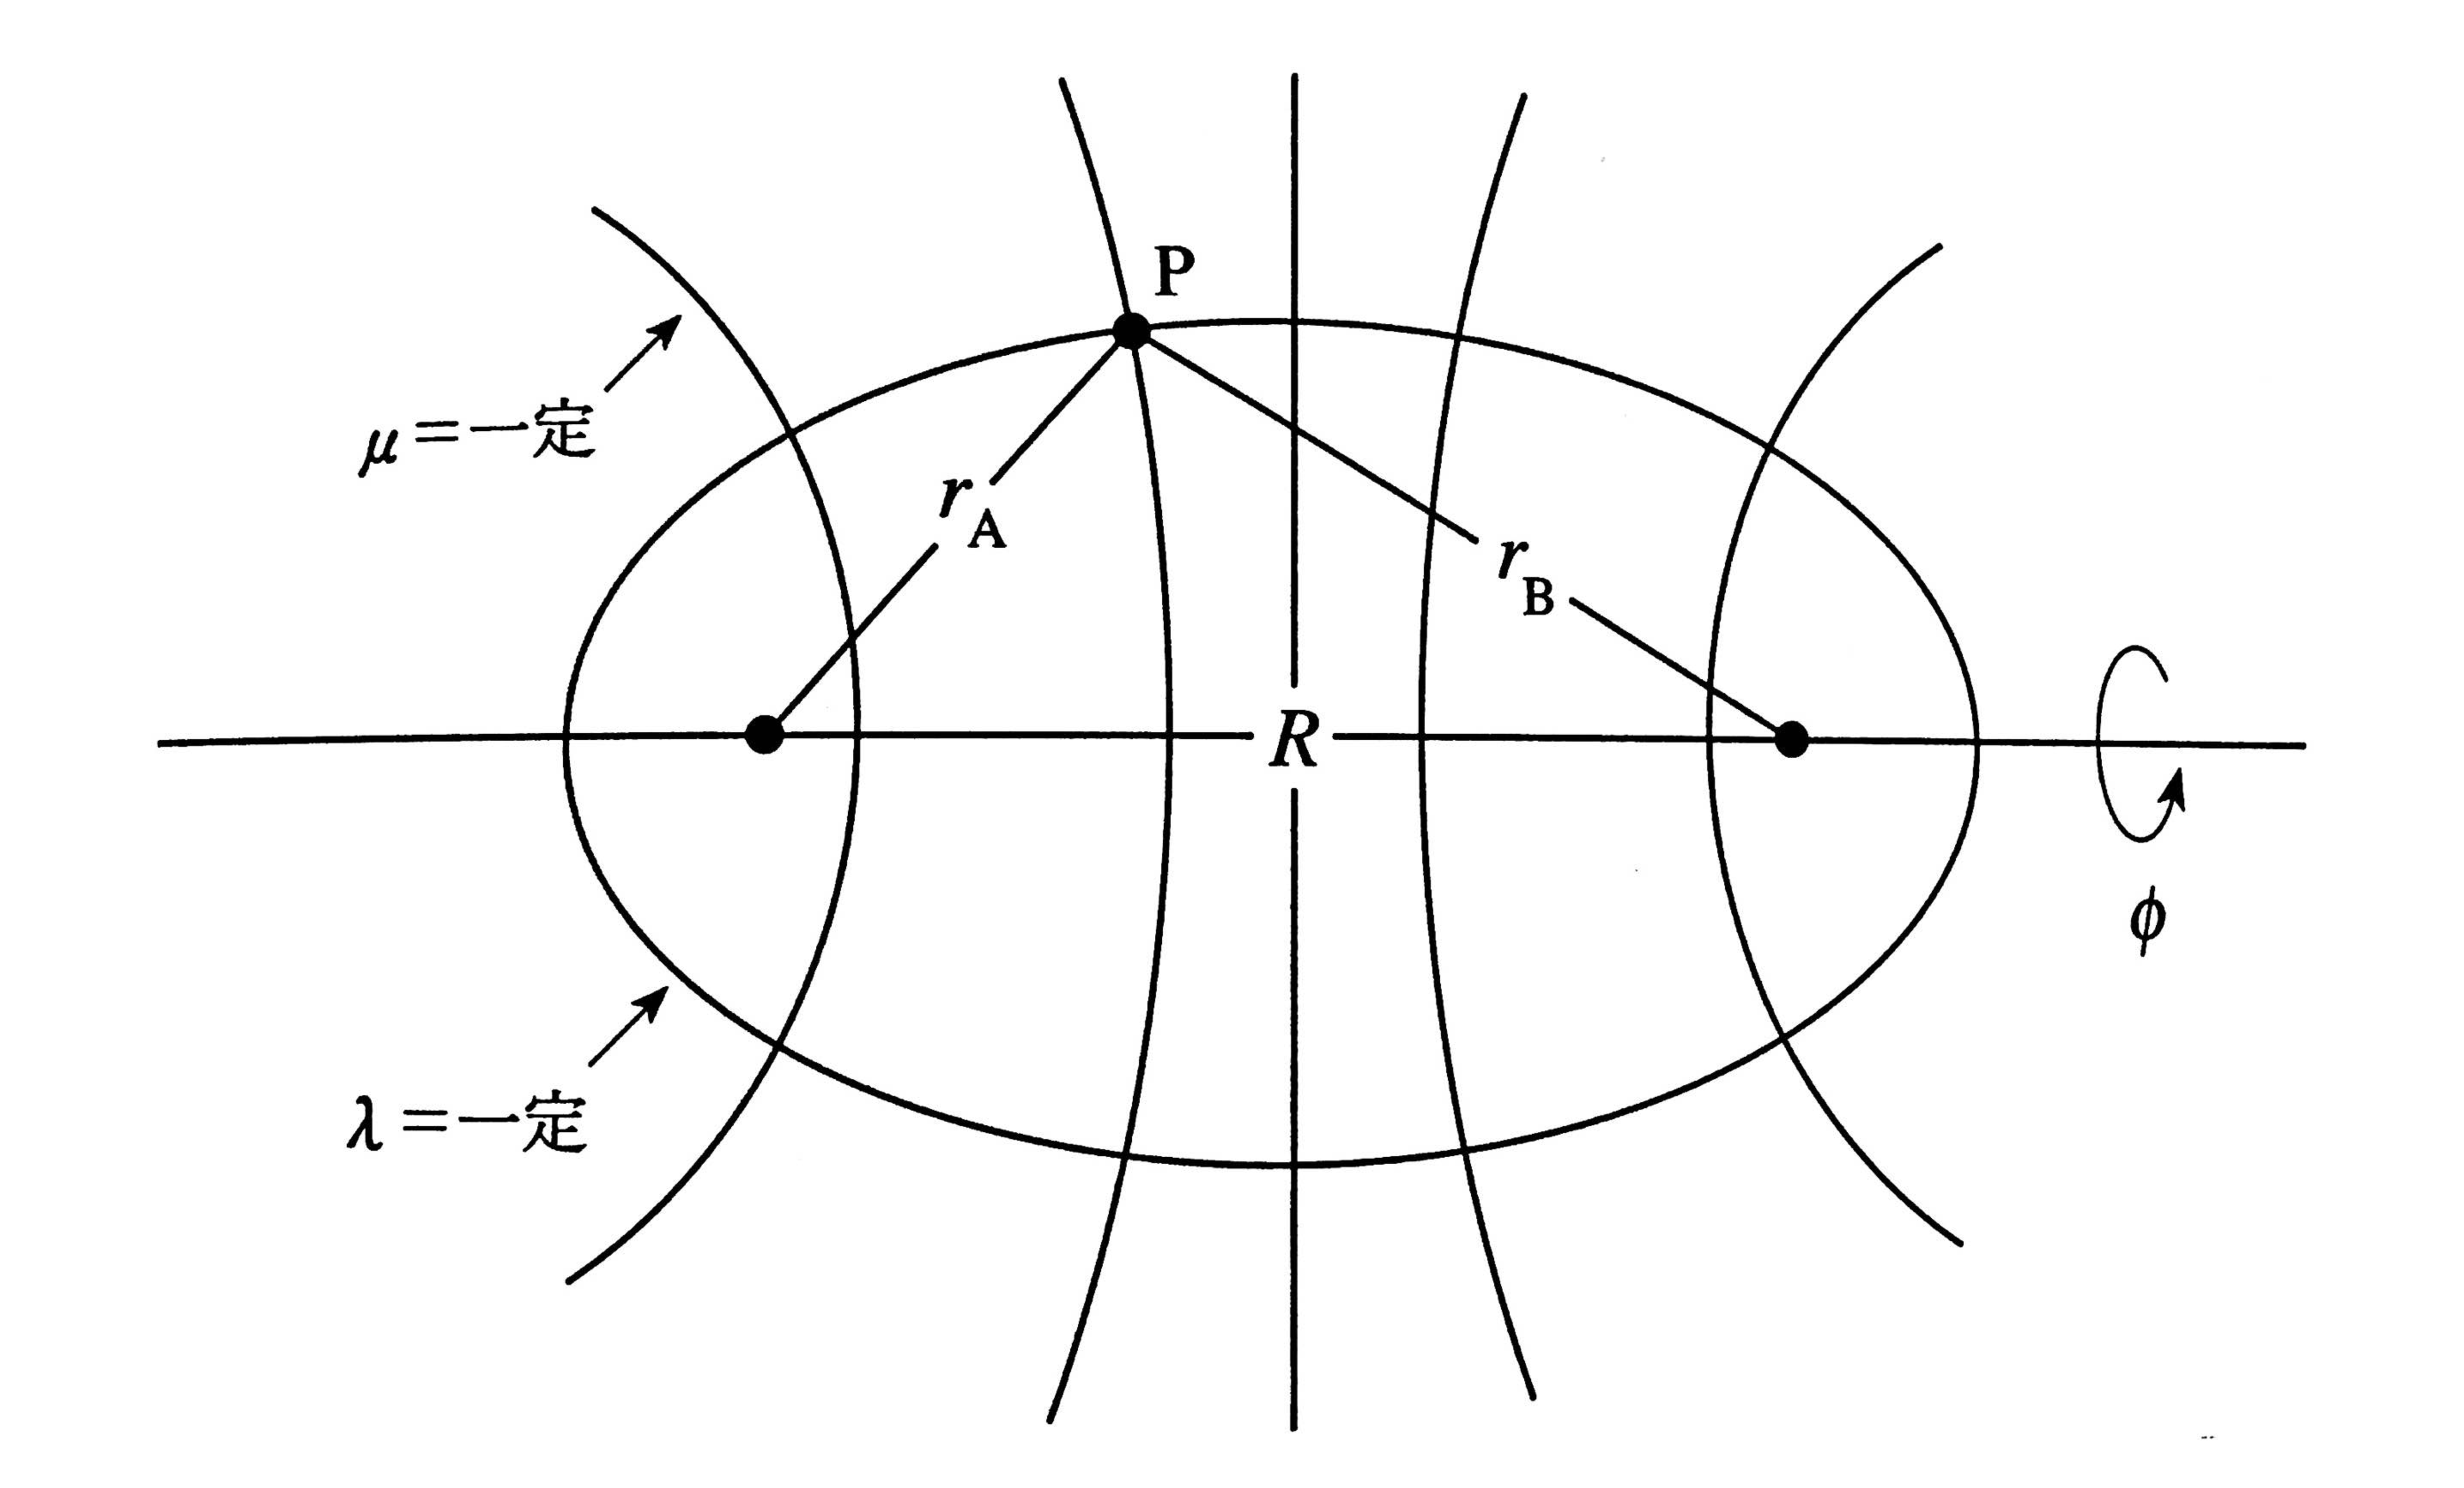
\includegraphics{elliptic.pdf}}
    %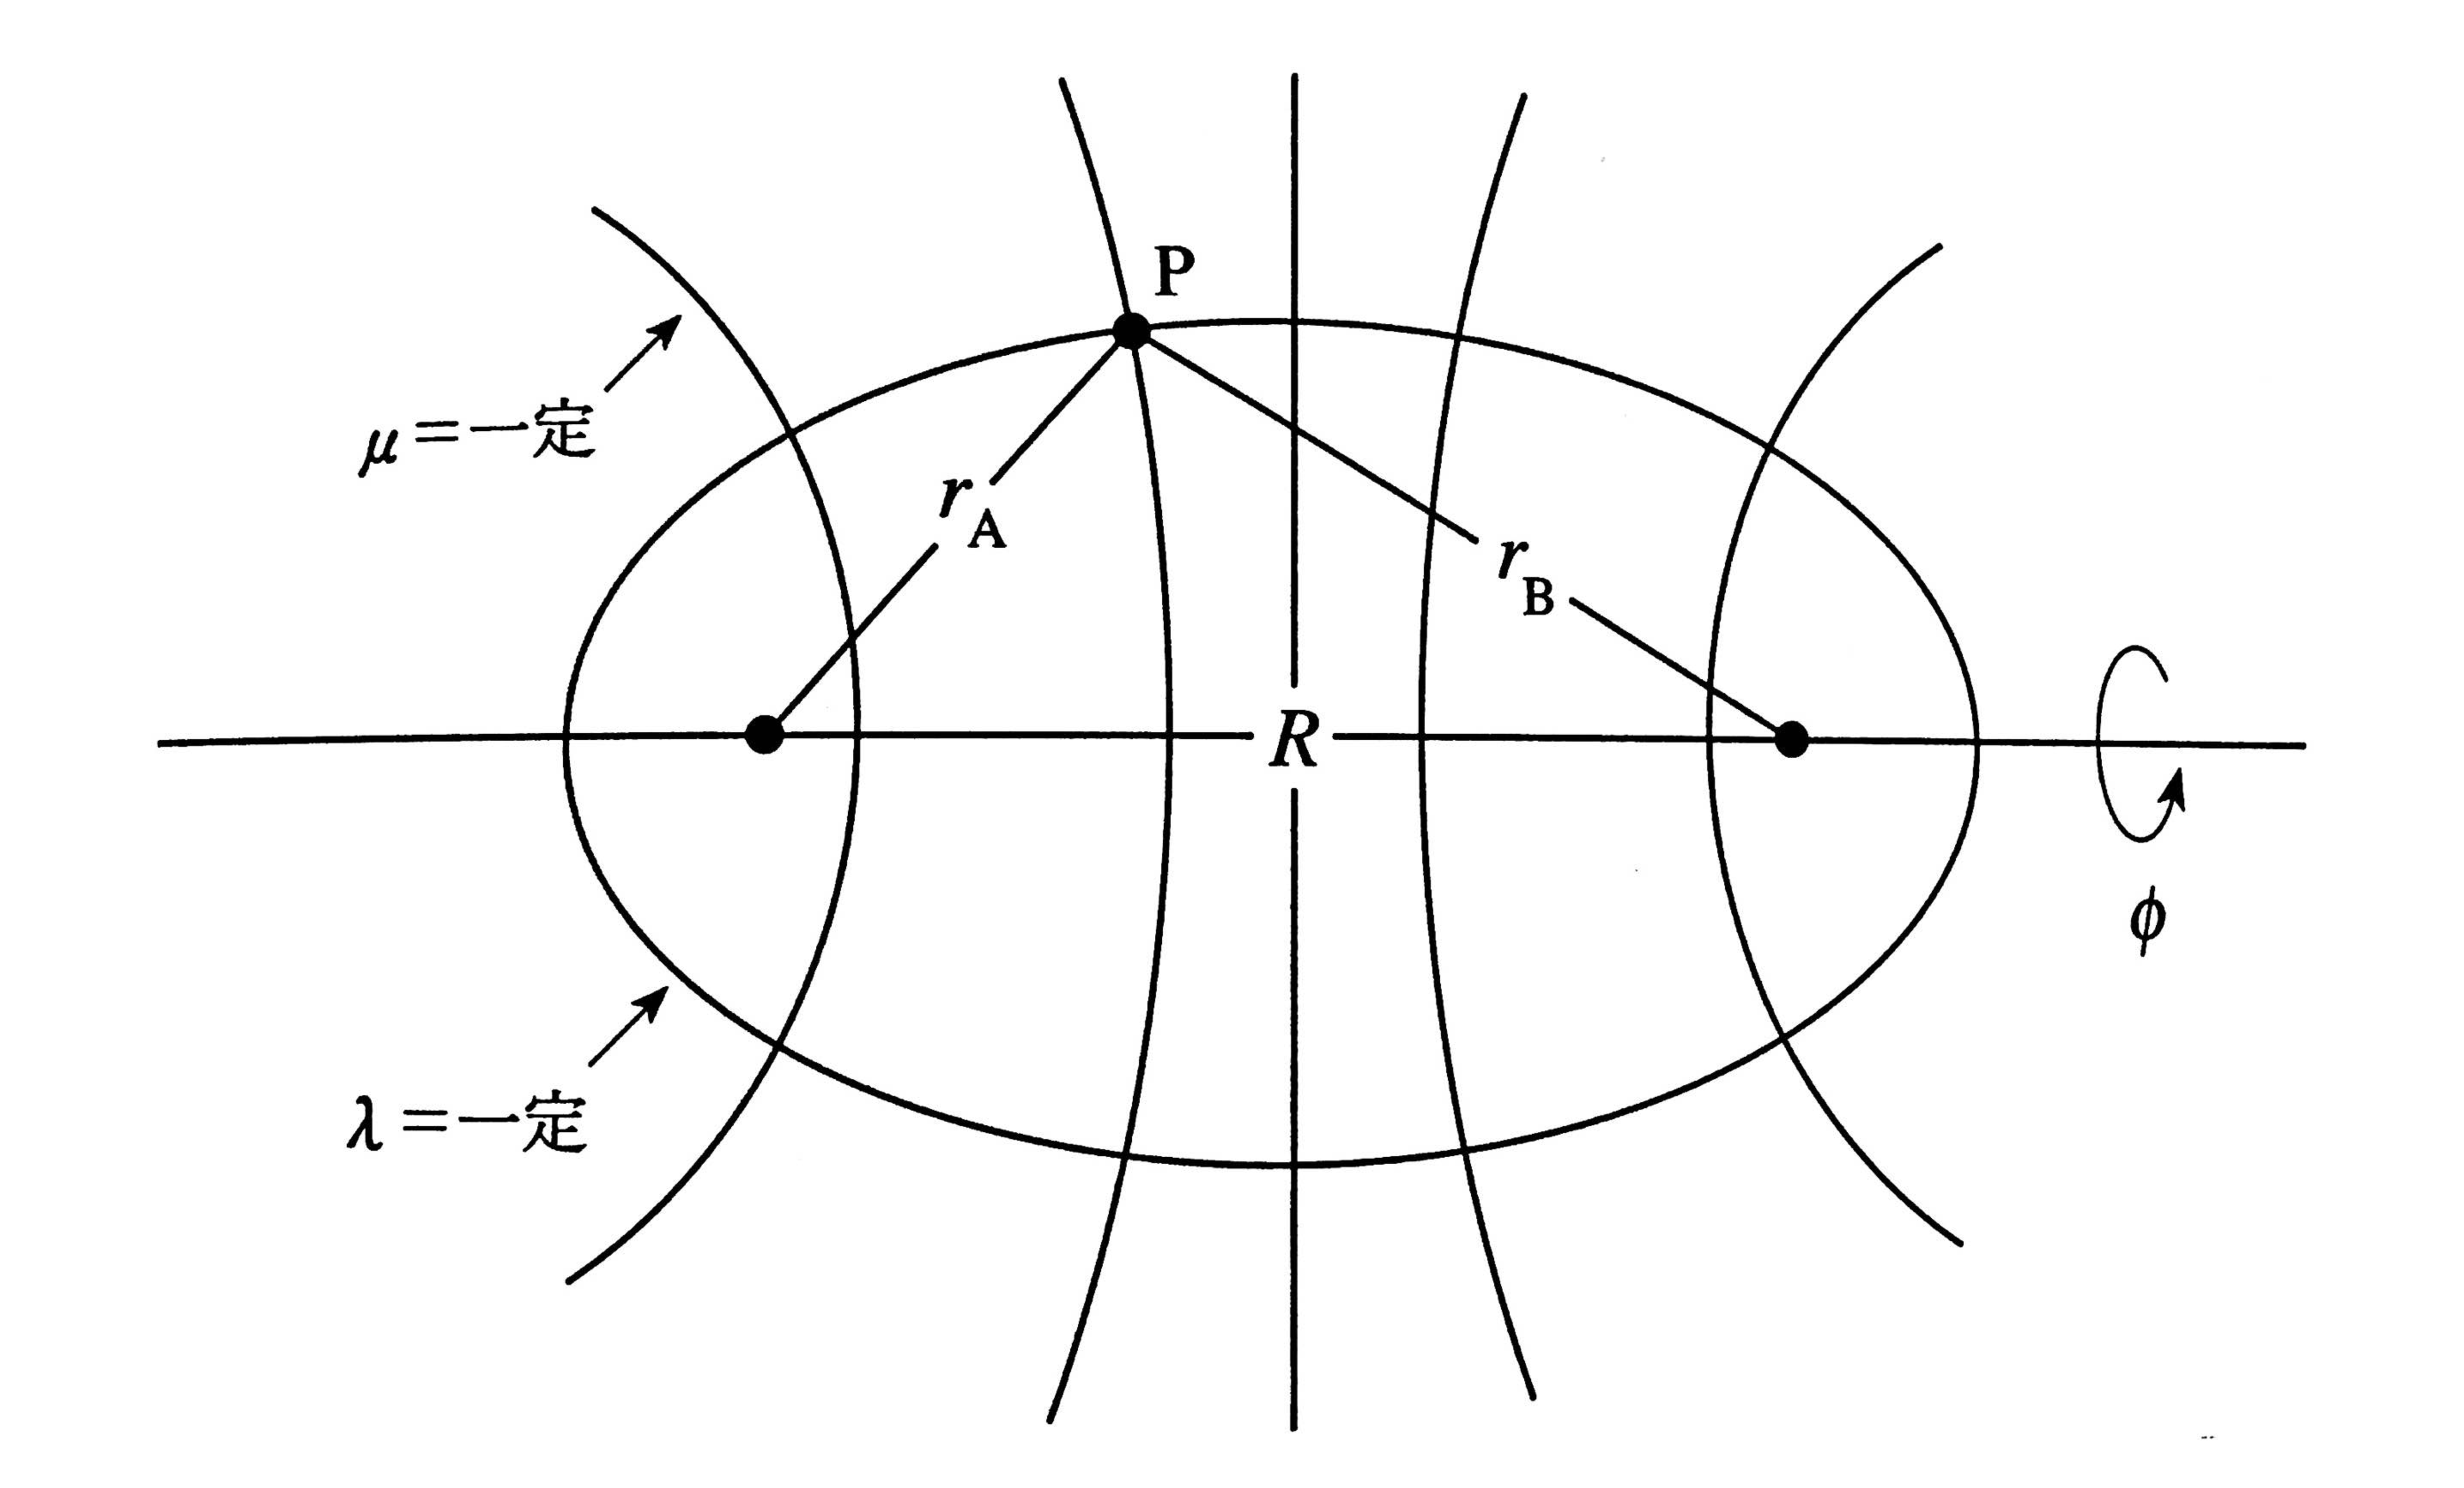
\includegraphics[scale=0.5]{elliptic.pdf}
    \caption{\label{fig:elliptic}
      {
        A volume element in elliptic corrdinate system is given as $d\mathbf{r}=\frac{R^3}{8}(\lambda^2-\mu^2)d\lambda d\mu d\phi$ where $\lambda$ and $\mu$ are defined as $\lambda=\frac{r_A+r_B}{R}$ and $\mu=\frac{r_A-r_B}{R}$. The integration ranges for $\lambda$, $\mu$ and $\phi$ are $1\leq \lambda<\infty$, $-1\leq\mu\leq 1$ and $0\leq\phi\leq 2\pi$, respectively.
      }
    }
    \end{center}
  \end{figure}
}

%\noindent
%{\bf 問い5} 式(\ref{eq:S})の積分を、変数変換で評価し、結果が問い3と一致することを示せ。

\noindent
{\bf 問い5}
水素分子イオンの反結合性軌道は
\begin{align}
  \Psi_{-}=C(\Phi_\text{A1s}-\Phi_\text{B1s})\label{eq:hanketugou}
\end{align}
と近似される。式(\ref{eq:hanketugou})から得られるエネルギーが
\begin{align}
  E_-=E_\text{1s}+\frac{J-K}{1-S}  
\end{align}
となることを示せ。
また、結合性及び反結合性軌道エネルギーは、水素原子の1s軌道エネルギーを基準として、Fig. \ref{fig:suiso}のようになる。結合性軌道のみが極小点を持つのは何故か。
このときクーロン積分J及び交換積分Kは核間距離Rの関数として
\begin{align}
  &J(R)=\exp(-2R)\left(1+\frac{1}{R}\right) \label{eq:J} \\
  &K(R)=\frac{S(R)}{R}-\exp(-R)\left(1+R\right) \label{eq:K}
\end{align}
と計算される。
{
  \begin{figure}[H]
    \begin{center}
    \scalebox{0.1}{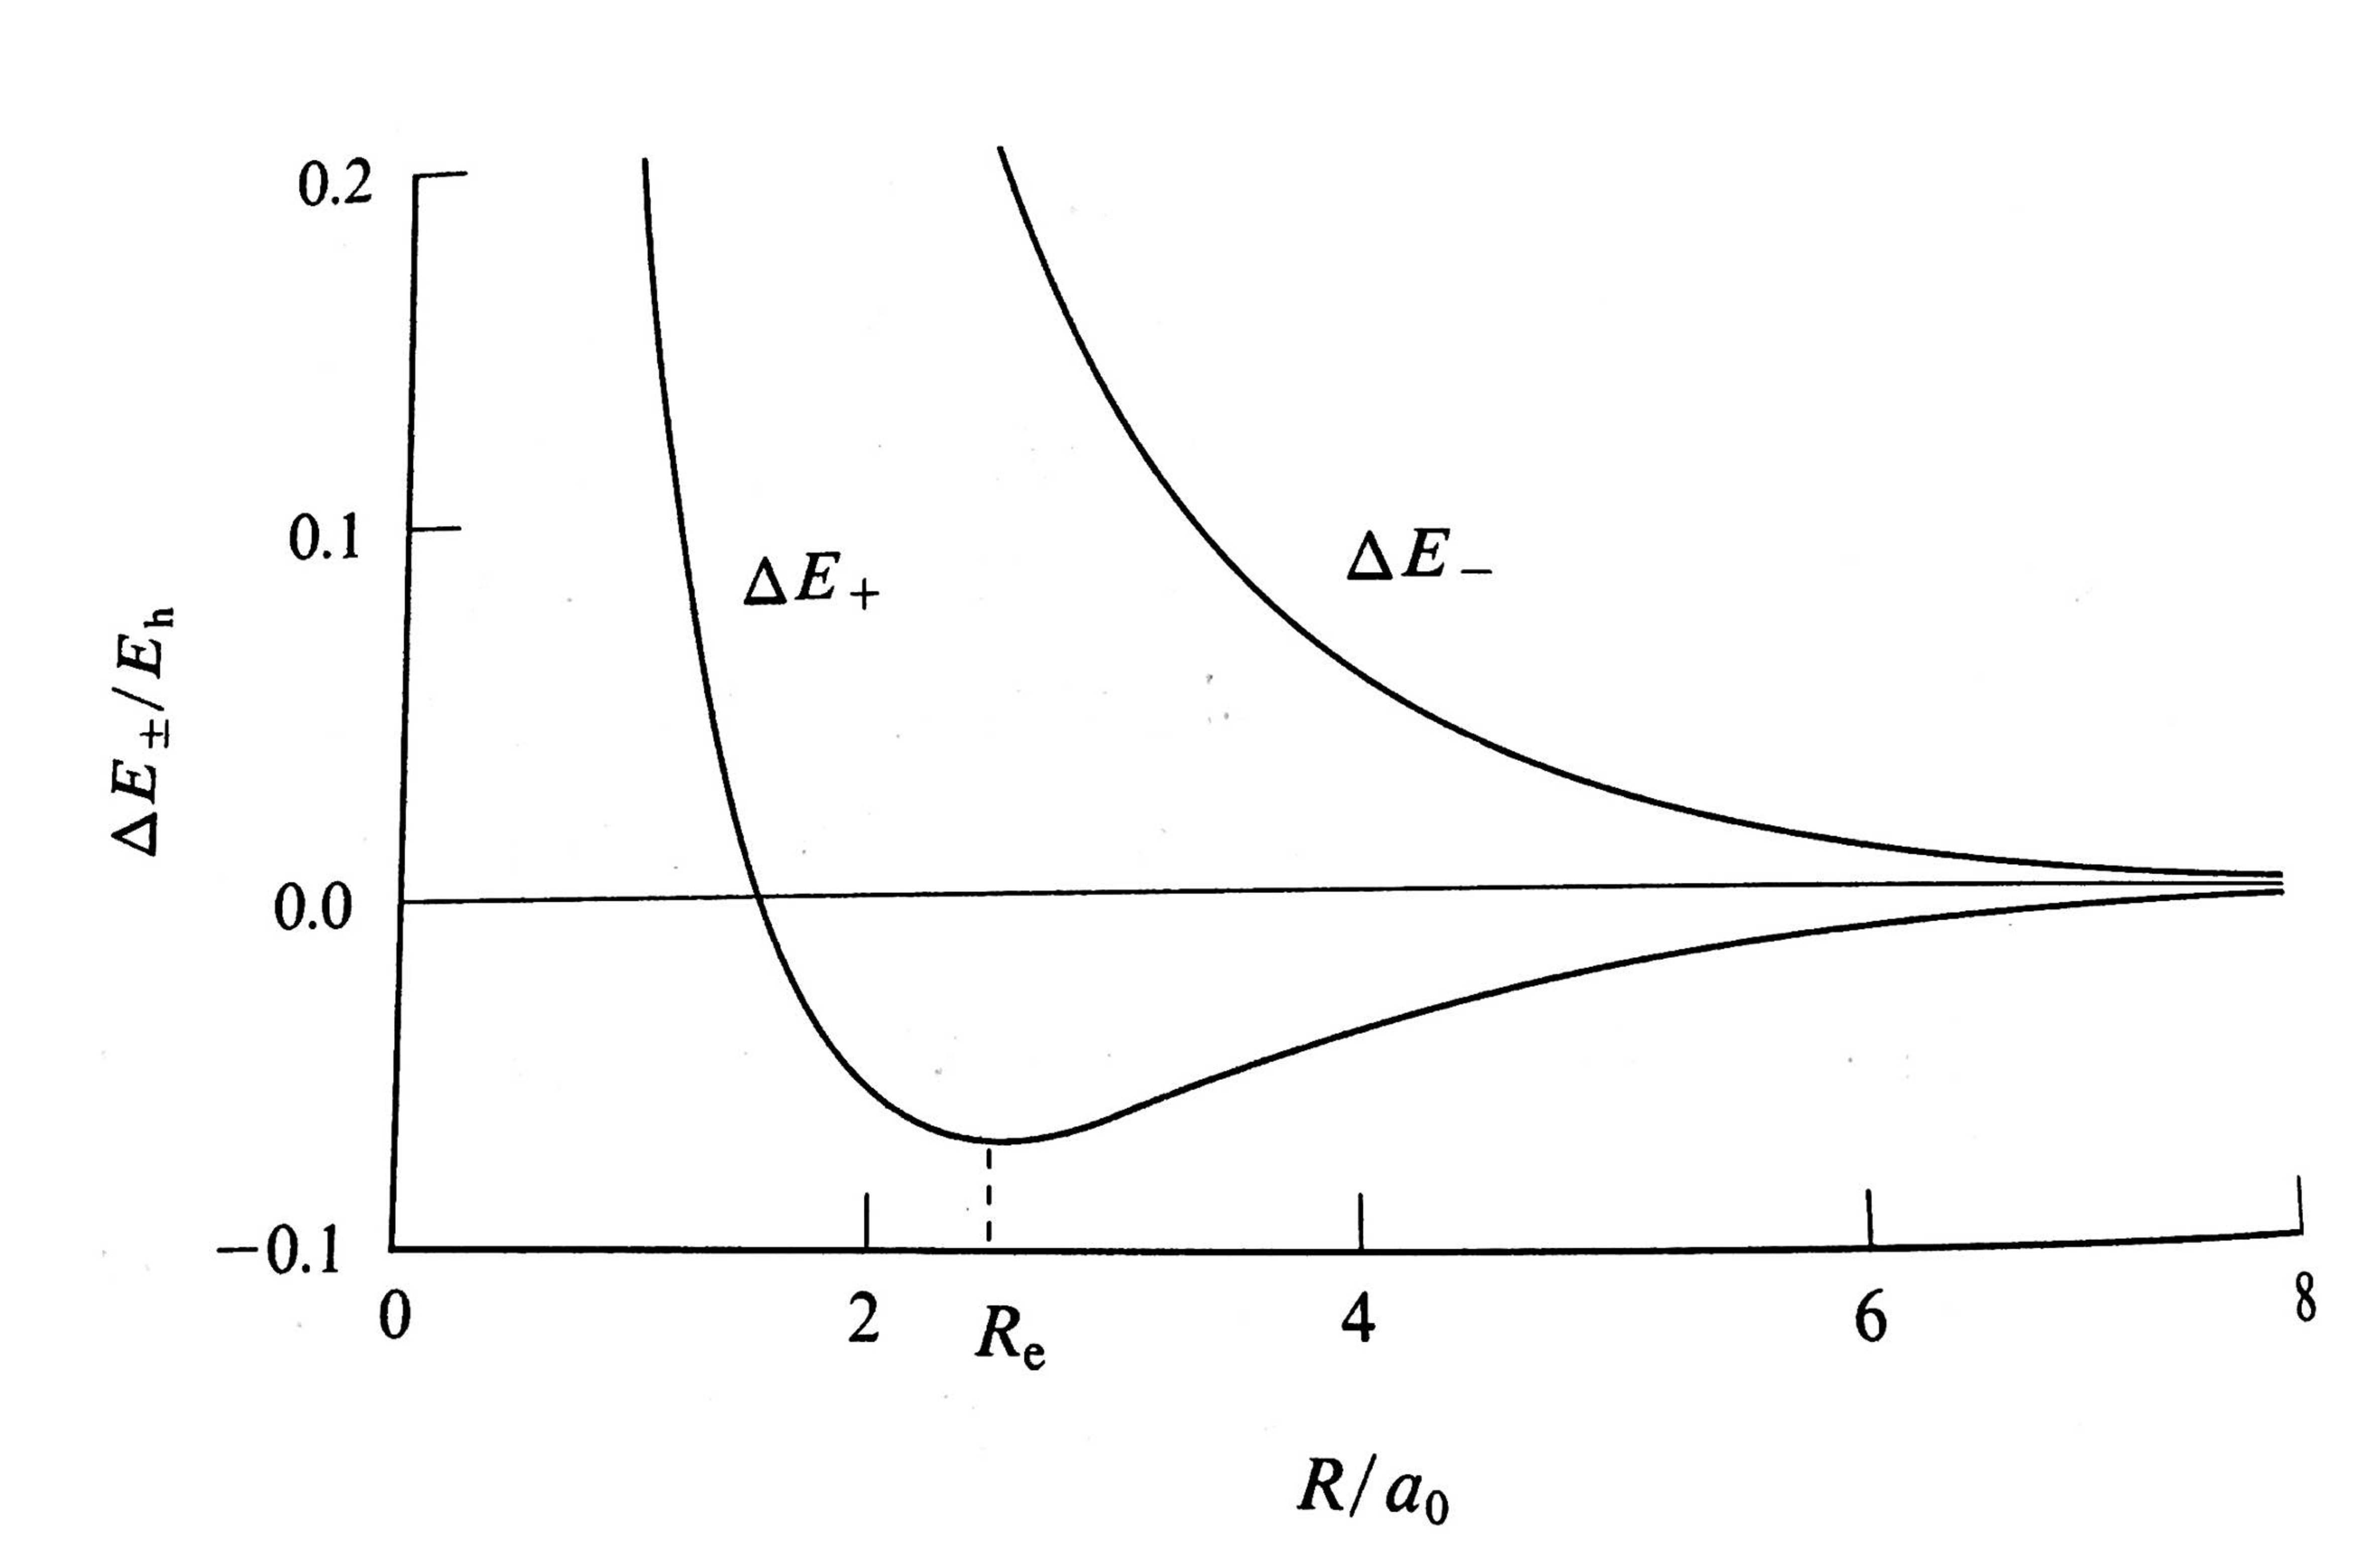
\includegraphics{hydrogen-ion.pdf}}
    \caption{\label{fig:suiso}
      {
        The potential energy curves for bonding ($\Delta \text{E}_+$) and anti-bonding ($\Delta \text{E}_-$) orbitals relative to hydrogen $1s$ state. The relative energy ($\Delta \text{E}_{\pm}$) is calculated as $\text{E}_{\pm} - E_{1s}$.
      }
    }
    \end{center}
  \end{figure}
}

\noindent
    {\bf 問題B.} 炭化水素化合物の$\pi$対称性を持つ分子軌道を単純H\"uckel法で計算する。単純H\"ckelモデルでは、$i$番目の$\pi$あるいは$\pi^*$分子軌道は、その分子を構成する炭素原子に中心を持つ$2p_z$軌道の線型結合で近似される。
\begin{align}
  |\psi_\pi^i\rangle=\sum_A^\text{Atoms}C^i_{2p_z\text{A}}|\psi_{2p_z\text{A}}\rangle \label{eq:hueckel}
\end{align}
式(\ref{eq:hueckel})における$C$-係数は変分的に決定される。単純H\"uckelモデルでは、以下の大胆な近似を導入する:
\begin{itemize}
\item Hamiltonian行列の対角要素 ($\langle\psi_{2p_z\text{A}}|H|\psi_{2p_z\text{A}}\rangle$) を単一の定数$\alpha$として近似。
\item 隣り合う原子上の$2p_z$軌道間のHamiltonian行列要素 ($\langle\psi_{2p_z\text{A}}|H|\psi_{2p_z\text{A+1}}\rangle$) を単一の定数$\beta$として近似。
\item 上記以外のHamiltonian行列要素は全て0とする。
\item $2p_z$軌道間の重なり行列は単位行列とする。
\end{itemize}

\noindent
{\bf 問い6} ベンゼンの$\pi$及び$\pi^*$軌道関数及び軌道エネルギーを求めよ。

\noindent
{\bf 問い7} シクロブタジエンの$\pi$及び$\pi^*$軌道関数及び軌道エネルギーを求めよ。シクロブタジエンの基底電子状態についてHundの規則を適用せよ。シクロブタジエンの安定性を2つの孤立エテン分子の安定性と比較せよ。

\noindent
{\bf 問い8} トリメチレンメタンの$\pi$及び$\pi^*$軌道関数及び軌道エネルギーを求めよ。トリメチルメタンの$\pi$軌道エネルギーを2つの孤立エテン分子のエネルギーと比較せよ。

\noindent
{\bf 問い9} ブタジエンの$\pi$及び$\pi^*$軌道関数及び軌道エネルギーを求めよ。またシクロブタジエンでは、$\pi$電子が均一に炭素原子上に分布していることを示せ。ここで原子$A$上の$\pi$電子密度は$q_A=\sum_i n_i |C^i_{2p_z\text{A}}|^2$と与えられる。ここで$n_i$は分子軌道$i$を占有する電子数である。

\noindent
{\bf 問い10} 原子A--B間の$\pi$結合次数は$P^\pi_{AB}=\sum_i n_i C^i_{2p_z\text{A}} C^i_{2p_z\text{B}}$と与えられる。ブタジエンについて$P^\pi_{12}=0.8942$及び$P^\pi_{23}=0.4473$となることを示せ。

\section{積分公式}
\begin{align}
  &\int x   \exp(ax) dx = \exp(ax)\left(\frac{x  }{a}-\frac{1}{a^2}\right) \\
  &\int x^2 \exp(ax) dx = \exp(ax)\left(\frac{x^2}{a}-\frac{2x}{a^2}+\frac{2}{a^3}\right) 
\end{align}

\section{さいごに}

誤植を発見した場合や、つじつまが合わない問題があった場合、齋藤までお知らせください。

\end{document}
